\documentclass[11pt,a4paper]{report}
\usepackage[textwidth=37em,vmargin=30mm]{geometry}
\usepackage{calc,xunicode,amsmath,amssymb,paralist,enumitem,tabu,booktabs,datetime2,xeCJK,xeCJKfntef,listings}
\usepackage{tocloft,fancyhdr,tcolorbox,xcolor,graphicx,eso-pic,xltxtra,xelatexemoji}

\newcommand{\envyear}[0]{2025}
\newcommand{\envdatestr}[0]{2025-05-27}
\newcommand{\envfinaldir}[0]{webdb/2025/20250527/final}

\usepackage[hidelinks]{hyperref}
\hypersetup{
    colorlinks=false,
    pdfpagemode=FullScreen,
    pdftitle={Web Digest - \envdatestr}
}

\setlength{\cftbeforechapskip}{10pt}
\renewcommand{\cftchapfont}{\rmfamily\bfseries\large\raggedright}
\setlength{\cftbeforesecskip}{2pt}
\renewcommand{\cftsecfont}{\sffamily\small\raggedright}

\setdefaultleftmargin{2em}{2em}{1em}{1em}{1em}{1em}

\usepackage{xeCJK,xeCJKfntef}
\xeCJKsetup{PunctStyle=plain,RubberPunctSkip=false,CJKglue=\strut\hskip 0pt plus 0.1em minus 0.05em,CJKecglue=\strut\hskip 0.22em plus 0.2em}
\XeTeXlinebreaklocale "zh"
\XeTeXlinebreakskip = 0pt


\setmainfont{Brygada 1918}
\setromanfont{Brygada 1918}
\setsansfont{IBM Plex Sans}
\setmonofont{JetBrains Mono NL}
\setCJKmainfont{Noto Serif CJK SC}
\setCJKromanfont{Noto Serif CJK SC}
\setCJKsansfont{Noto Sans CJK SC}
\setCJKmonofont{Noto Sans CJK SC}

\setlength{\parindent}{0pt}
\setlength{\parskip}{8pt}
\linespread{1.15}

\lstset{
	basicstyle=\ttfamily\footnotesize,
	numbersep=5pt,
	backgroundcolor=\color{black!5},
	showspaces=false,
	showstringspaces=false,
	showtabs=false,
	tabsize=2,
	captionpos=b,
	breaklines=true,
	breakatwhitespace=true,
	breakautoindent=true,
	linewidth=\textwidth
}






\newcommand{\coverpic}[2]{
    % argv: itemurl, authorname
    Cover photo by #2~~(\href{#1}{#1})
}
\newcommand{\makeheader}[0]{
    \begin{titlepage}
        % \newgeometry{hmargin=15mm,tmargin=21mm,bmargin=12mm}
        \begin{center}
            
            \rmfamily\scshape
            \fontspec{BaskervilleF}
            \fontspec{Old Standard}
            \fontsize{59pt}{70pt}\selectfont
            WEB\hfill DIGEST
            
            \vfill
            % \vskip 30pt
            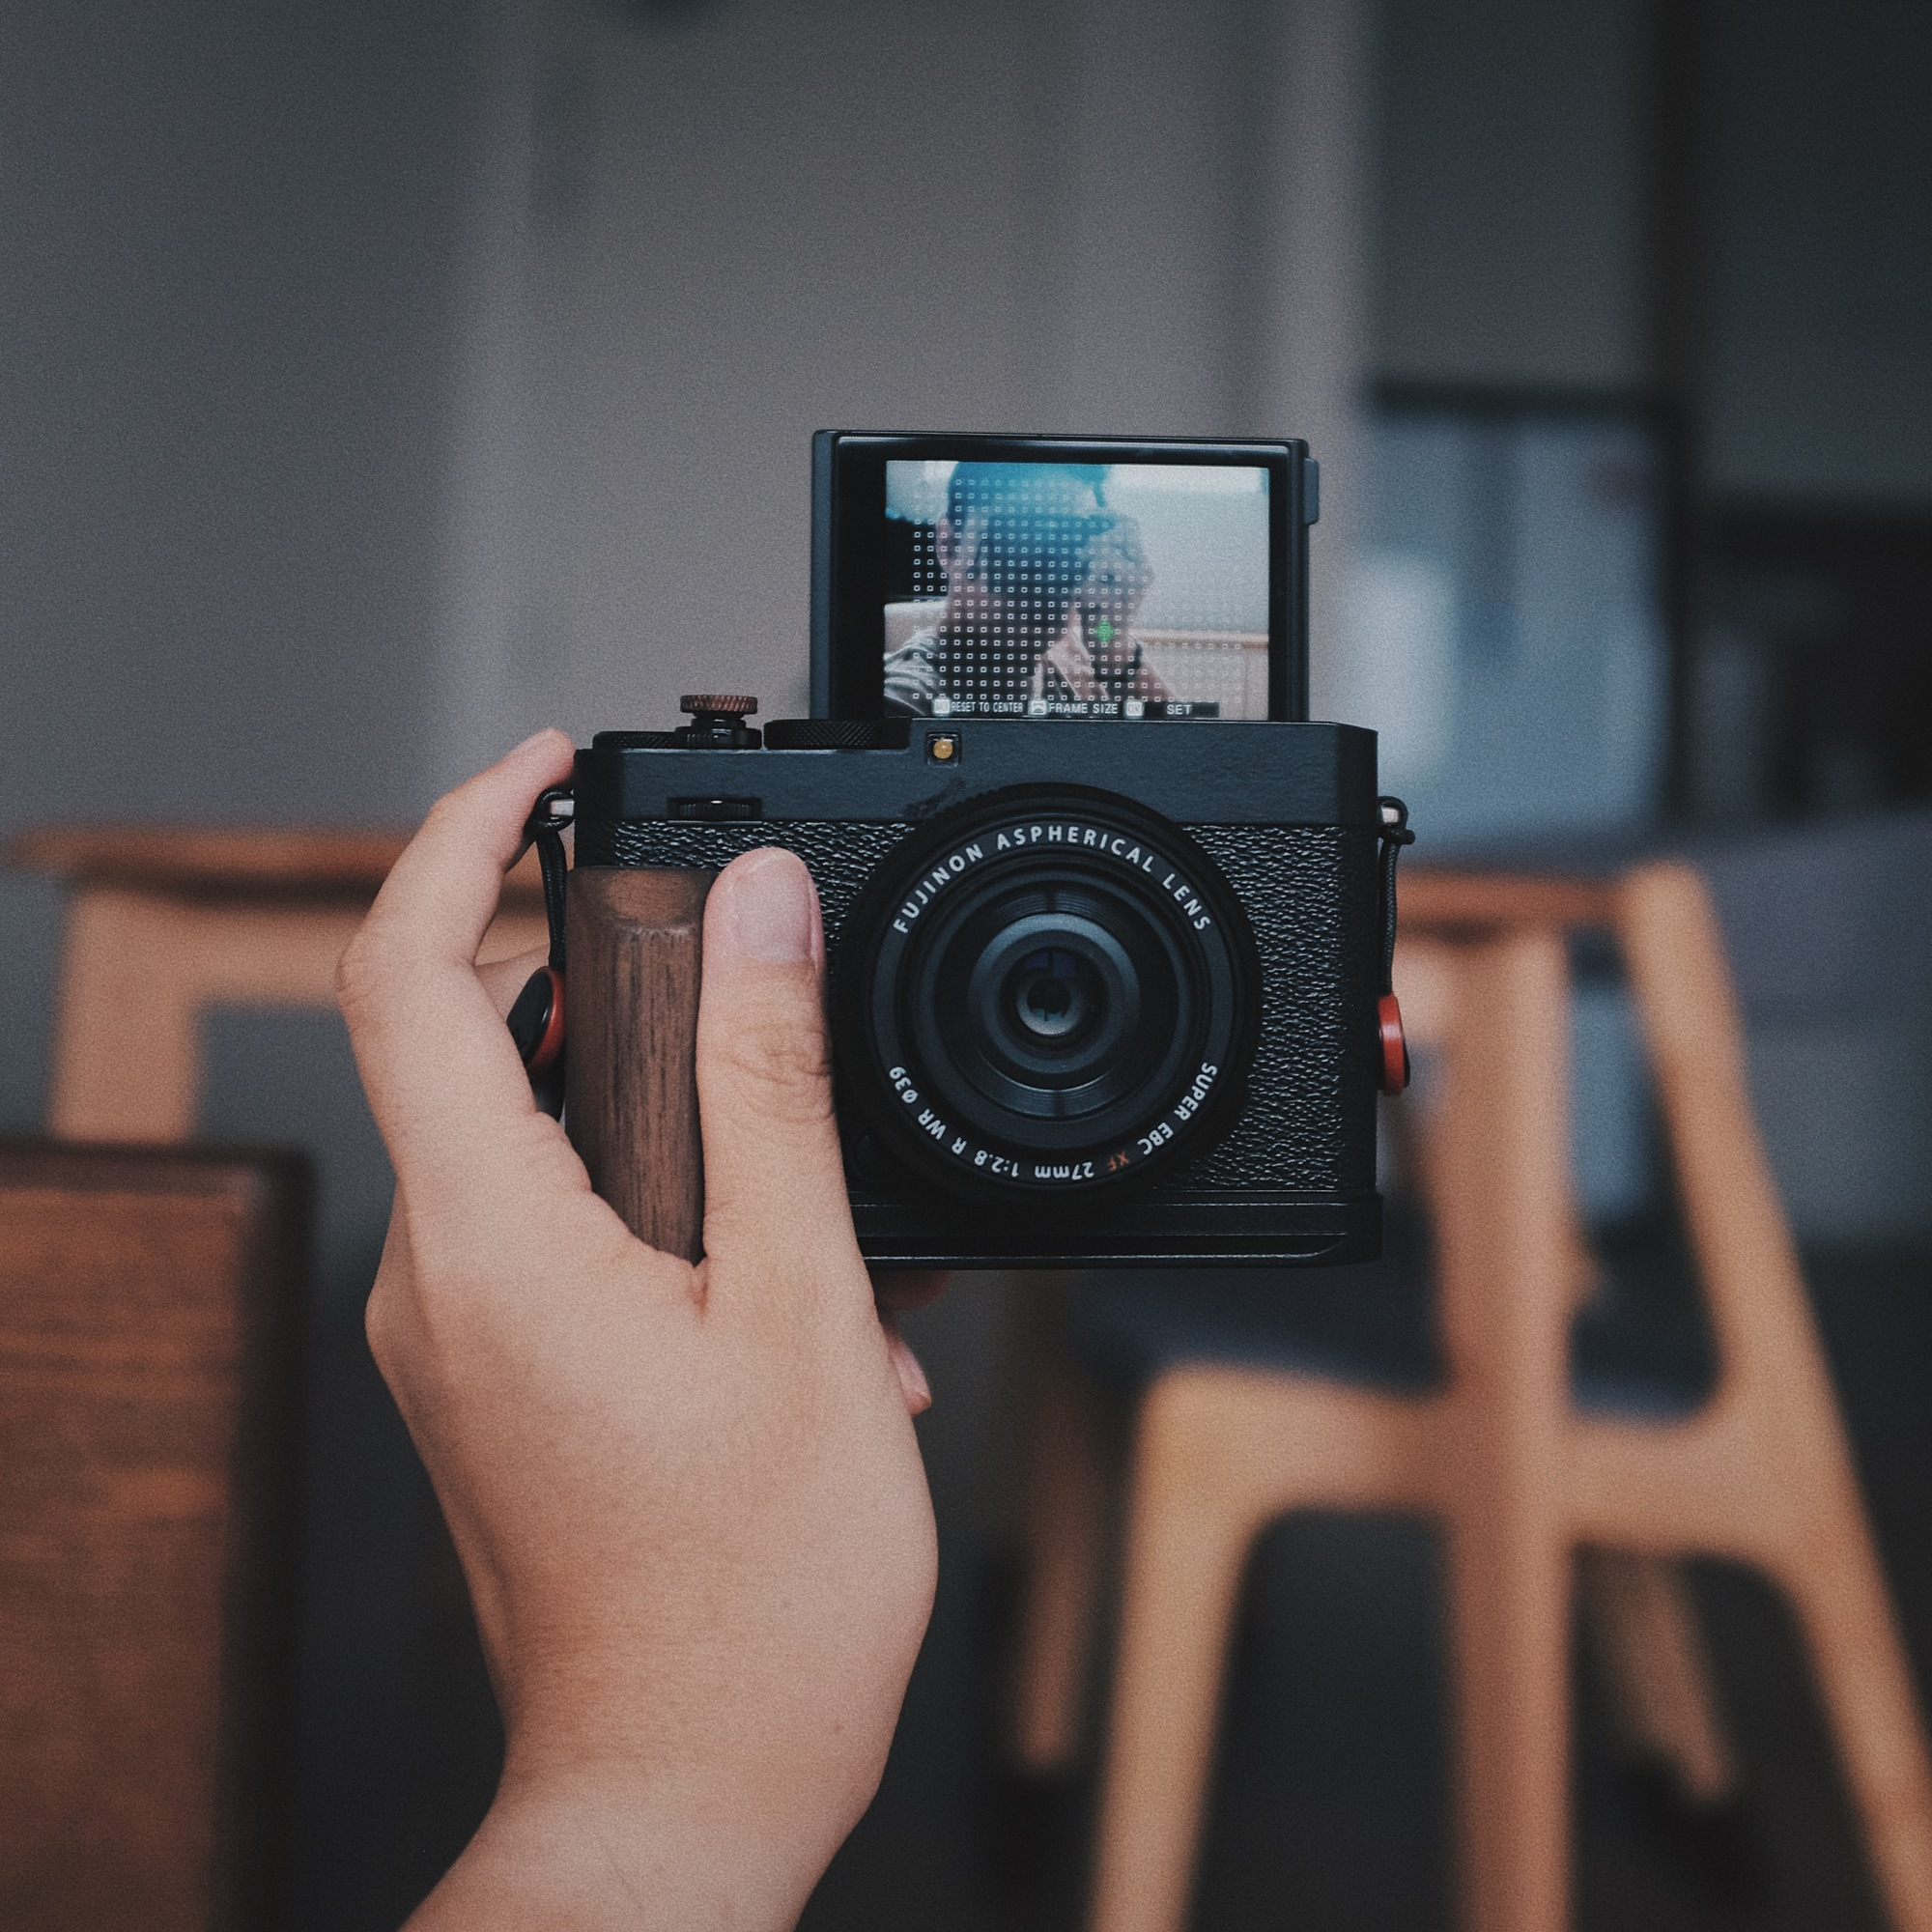
\includegraphics[width=\linewidth]{\envfinaldir/coverpic-prod.jpg}\par
            % \vskip 30pt
            \vfill

            \normalsize\rmfamily\scshape
            \copyright{} The Web Digest Project \hfill\large \envdatestr
        \end{center}
    \end{titlepage}
    % \restoregeometry
}
\newcommand{\simplehref}[1]{%
    \textcolor{blue!80!green}{\href{#1}{#1}}%
}
\renewcommand{\contentsname}{\center\Huge\sffamily\bfseries Contents\par\vskip 20pt}
\newcounter{ipartcounter}
\setcounter{ipartcounter}{0}
\newcommand{\ipart}[1]{
    % \vskip 20pt
    \clearpage
    \stepcounter{ipartcounter}
    \phantomsection
    \addcontentsline{toc}{chapter}{#1}
    % \begin{center}
    %     \Huge
    %     \sffamily\bfseries
    %     #1
    % \end{center}
    % \vskip 20pt plus 7pt
}
\newcounter{ichaptercounter}
\setcounter{ichaptercounter}{0}
\newcommand{\ichapter}[1]{
    % \vskip 20pt
    \clearpage
    \stepcounter{ichaptercounter}
    \phantomsection
    \addcontentsline{toc}{section}{\numberline{\arabic{ichaptercounter}}#1}
    \begin{center}
        \Huge
        \sffamily\bfseries
        #1
    \end{center}
    \vskip 20pt plus 7pt
}
\newcommand{\entrytitlefont}[1]{\subsection*{\raggedright\Large\sffamily\bfseries#1}}
\newcommand{\entryitemGeneric}[2]{
    % argv: title, url
    \parbox{\linewidth}{
        \entrytitlefont{#1}\par\vskip 5pt
        \footnotesize\ttfamily\mdseries
        \simplehref{#2}
    }\vskip 11pt plus 11pt minus 1pt
}
\newcommand{\entryitemGithub}[3]{
    % argv: title, url, desc
    \parbox{\linewidth}{
        \entrytitlefont{#1}\par\vskip 5pt
        \footnotesize\ttfamily\mdseries
        \simplehref{#2}\par\vskip 5pt
        \small\rmfamily\mdseries#3
    }\vskip 11pt plus 11pt minus 1pt
}
\newcommand{\entryitemAp}[3]{
    % argv: title, url, desc
    \parbox{\linewidth}{
        \entrytitlefont{#1}\par\vskip 5pt
        \footnotesize\ttfamily\mdseries
        \simplehref{#2}\par\vskip 5pt
        \small\rmfamily\mdseries#3
    }\vskip 11pt plus 11pt minus 1pt
}
\newcommand{\entryitemHackernews}[3]{
    % argv: title, hnurl, rawurl
    % \parbox{\linewidth}{
    %     \entrytitlefont{#1}\par\vskip 5pt
    %     \footnotesize\ttfamily\mdseries
    %     \simplehref{#3}\par
    %     \textcolor{black!50}{\href{#2}{#2}}
    % }\vskip 11pt plus 11pt minus 1pt
    \begin{minipage}{\linewidth}
            \entrytitlefont{#1}\par\vskip 5pt
            \footnotesize\ttfamily\mdseries
            \simplehref{#3}\par
            \textcolor{black!50}{\href{#2}{#2}}
    \end{minipage}\par\vskip 11pt plus 11pt minus 1pt
}







\begin{document}

\makeheader

\tableofcontents\clearpage




\ipart{Developers}
\ichapter{Hacker News}
\entryitemTwoLinks{Owls in Towels}{https://news.ycombinator.com/item?id=44101349}{https://owlsintowels.org/}

\entryitemTwoLinks{Britain's police are restricting speech in worrying ways}{https://news.ycombinator.com/item?id=44100552}{https://www.economist.com/britain/2025/05/15/britains-police-are-restricting-speech-in-worrying-ways}

\entryitemTwoLinks{Lossless video compression using Bloom filters}{https://news.ycombinator.com/item?id=44100179}{https://github.com/ross39/new\_bloom\_filter\_repo/blob/main/README.md}

\entryitemTwoLinks{CSS Minecraft}{https://news.ycombinator.com/item?id=44100148}{https://benjaminaster.com/css-minecraft/}

\entryitemTwoLinks{Claude 4 and GitHub MCP will leak your private GitHub repositories}{https://news.ycombinator.com/item?id=44100082}{https://twitter.com/lbeurerkellner/status/1926991491735429514}

\entryitemTwoLinks{Duolingo CEO tries to walk back AI-first comments, fails}{https://news.ycombinator.com/item?id=44100035}{https://htxt.co.za/2025/05/duolingo-ceo-tries-to-walk-back-ai-first-comments-fails/}

\entryitemTwoLinks{TSMC bets on unorthodox optical tech}{https://news.ycombinator.com/item?id=44099407}{https://spectrum.ieee.org/microled-optical-chiplet}

\entryitemTwoLinks{Show HN: PgDog – Shard Postgres without extensions}{https://news.ycombinator.com/item?id=44099187}{https://github.com/pgdogdev/pgdog}

\entryitemTwoLinks{TeleMessage Customers Include DC Police, Andreessen Horowitz, JP Morgan,Hundreds}{https://news.ycombinator.com/item?id=44099096}{https://micahflee.com/telemessage-customers-include-dc-police-andreesen-horowitz-jp-morgan-and-hundreds-more/}

\entryitemTwoLinks{Data breach exposes 184M passwords, likely captured by malware}{https://news.ycombinator.com/item?id=44099008}{https://www.zdnet.com/article/massive-data-breach-exposes-184-million-passwords-for-google-microsoft-facebook-and-more/}

\entryitemTwoLinks{Hacker News now runs on top of Common Lisp}{https://news.ycombinator.com/item?id=44099006}{https://lisp-journey.gitlab.io/blog/hacker-news-now-runs-on-top-of-common-lisp/}

\entryitemTwoLinks{I think it's time to give Nix a chance}{https://news.ycombinator.com/item?id=44098605}{https://maych.in/blog/its-time-to-give-nix-a-chance/}

\entryitemTwoLinks{Cloudflare CEO: Football piracy blocks will claim lives}{https://news.ycombinator.com/item?id=44098273}{https://torrentfreak.com/cloudflare-ceo-football-piracy-blocks-will-claim-lives-i-pray-no-one-dies-250526/}

\entryitemTwoLinks{German court sends VW execs to prison over Dieselgate scandal}{https://news.ycombinator.com/item?id=44098091}{https://www.politico.eu/article/german-court-vw-execs-prison-dieselgate-scandal-volkswagen-environment-illegal-pollution/}

\entryitemTwoLinks{Google is burying the web alive}{https://news.ycombinator.com/item?id=44097490}{https://nymag.com/intelligencer/article/google-ai-mode-search-results-bury-the-web.html}

\entryitemTwoLinks{A new class of materials that can passively harvest water from air}{https://news.ycombinator.com/item?id=44097144}{https://blog.seas.upenn.edu/penn-engineers-discover-a-new-class-of-materials-that-passively-harvest-water-from-air/}

\entryitemTwoLinks{Particle Life simulation in browser using WebGPU}{https://news.ycombinator.com/item?id=44096808}{https://lisyarus.github.io/blog/posts/particle-life-simulation-in-browser-using-webgpu.html}

\entryitemTwoLinks{TIL: timeout in Bash scripts}{https://news.ycombinator.com/item?id=44096395}{https://heitorpb.github.io/bla/timeout/}

\entryitemTwoLinks{The double standard of webhook security and API security}{https://news.ycombinator.com/item?id=44096251}{https://www.speakeasy.com/blog/webhook-security}

\entryitemTwoLinks{Sleep apnea pill shows striking success in large clinical trial}{https://news.ycombinator.com/item?id=44095866}{https://www.science.org/content/article/sleep-apnea-pill-shows-striking-success-large-clinical-trial}\ichapter{Phoronix}
\entryitemGeneric{\hskip 0pt{}Linux 6.16 Adds Ability For Power Code To Freeze The File-System For Suspend \& Hibernate}{https://www.phoronix.com/news/Linux-6.16-Filesystem-Freezing}

\entryitemGeneric{\hskip 0pt{}New Linux Patches Properly Handle The Audio Jack On Sony's PS5 DualSense Controller}{https://www.phoronix.com/news/Sony-PS5-DualSense-Audio-Jack}

\entryitemGeneric{\hskip 0pt{}GNU Linux-libre 6.15-gnu Neuters The New NOVA NVIDIA Driver}{https://www.phoronix.com/news/GNU-Linux-Libre-6.15-gnu}

\entryitemGeneric{\hskip 0pt{}Armbian 25.5 Adds Support For Newer Single Board Computers}{https://www.phoronix.com/news/Armbian-25.5-Released}

\entryitemGeneric{\hskip 0pt{}Rust Makes Progress On Async Rust Experience, Stabilizing Tooling For Rust In The Kernel}{https://www.phoronix.com/news/Rust-Projects-Mid-2025}

\entryitemGeneric{\hskip 0pt{}New AMD SPI Driver Going Upstream In Linux 6.16}{https://www.phoronix.com/news/Linux-6.16-SPI}

\entryitemGeneric{\hskip 0pt{}Firefox 139.0 Now Available With Faster HTTP/3 Upload Performance}{https://www.phoronix.com/news/Firefox-139-Downloads}

\entryitemGeneric{\hskip 0pt{}Bcachefs: Performance Improvements, Recovery Work \& Nicer Error Messages For Linux 6.16}{https://www.phoronix.com/news/Linux-6.16-Bcachefs}

\entryitemGeneric{\hskip 0pt{}POWER CPUs Ready With Dynamic Preemption For Linux 6.16}{https://www.phoronix.com/news/POWER-Dynamic-Preempt-Linux-616}\ichapter{Dribbble}
\entryitemGeneric{\hskip 0pt{}Stanley // Website}{https://dribbble.com/shots/26056691-Stanley-Website}

\entryitemGeneric{\hskip 0pt{}AltSocial}{https://dribbble.com/shots/26060858-AltSocial}

\entryitemGeneric{\hskip 0pt{}i SEA you}{https://dribbble.com/shots/26062936-i-SEA-you}

\entryitemGeneric{\hskip 0pt{}Glassmorphic 3D Logo Animation}{https://dribbble.com/shots/26061835-Glassmorphic-3D-Logo-Animation}

\entryitemGeneric{\hskip 0pt{}Meditation App Branding Concept}{https://dribbble.com/shots/26057810-Meditation-App-Branding-Concept}

\entryitemGeneric{\hskip 0pt{}Landing Page for an AI-Powered Design System}{https://dribbble.com/shots/26057663-Landing-Page-for-an-AI-Powered-Design-System}

\entryitemGeneric{\hskip 0pt{}Medic H - Logo Design}{https://dribbble.com/shots/26057472-Medic-H-Logo-Design}

\entryitemGeneric{\hskip 0pt{}Smart Home App}{https://dribbble.com/shots/26056748-Smart-Home-App}

\entryitemGeneric{\hskip 0pt{}Sellin dashboard}{https://dribbble.com/shots/26037015-Sellin-dashboard}

\entryitemGeneric{\hskip 0pt{}Fariland Headwear}{https://dribbble.com/shots/26058705-Fariland-Headwear}

\entryitemGeneric{\hskip 0pt{}Illustration}{https://dribbble.com/shots/26052539-Illustration}

\entryitemGeneric{\hskip 0pt{}Travel Startup Branding for Holidu: visual identity brand design}{https://dribbble.com/shots/25983747-Travel-Startup-Branding-for-Holidu-visual-identity-brand-design}

\entryitemGeneric{\hskip 0pt{}Playground web interaction}{https://dribbble.com/shots/26048246-Playground-web-interaction}

\entryitemGeneric{\hskip 0pt{}Onday - Logo Design}{https://dribbble.com/shots/26053436-Onday-Logo-Design}

\entryitemGeneric{\hskip 0pt{}Burger Time!}{https://dribbble.com/shots/26053795-Burger-Time}

\entryitemGeneric{\hskip 0pt{}Homepage Design — WoodNest}{https://dribbble.com/shots/26051400-Homepage-Design-WoodNest}

\entryitemGeneric{\hskip 0pt{}Magus Brand Identity Design}{https://dribbble.com/shots/26052344-Magus-Brand-Identity-Design}

\entryitemGeneric{\hskip 0pt{}Mighty Sketches}{https://dribbble.com/shots/26034483-Mighty-Sketches}

\entryitemGeneric{\hskip 0pt{}DICH™ Fashion Vol.2}{https://dribbble.com/shots/26046875-DICH-Fashion-Vol-2}

\entryitemGeneric{\hskip 0pt{}Account Dropdown}{https://dribbble.com/shots/26047665-Account-Dropdown}

\entryitemGeneric{\hskip 0pt{}L'Renee \& Associates logo}{https://dribbble.com/shots/26047943-L-Renee-Associates-logo}

\entryitemGeneric{\hskip 0pt{}Magus Logo Design}{https://dribbble.com/shots/26048055-Magus-Logo-Design}

\entryitemGeneric{\hskip 0pt{}Chromix – Logo Design // For Sale}{https://dribbble.com/shots/26048061-Chromix-Logo-Design-For-Sale}

\entryitemGeneric{\hskip 0pt{}Indonesia Travel Poster}{https://dribbble.com/shots/26049146-Indonesia-Travel-Poster}


\ipart{Developers~~~~(zh-Hans)}
\ichapter{Solidot}
\entryitemGeneric{\hskip 0pt{}英伟达准备推出新款中国专用 AI 芯片}{https://www.solidot.org/story?sid=81393}

\entryitemGeneric{\hskip 0pt{}木星早期大小是目前的两倍}{https://www.solidot.org/story?sid=81392}

\entryitemGeneric{\hskip 0pt{}天文学家发现黏在一起的双星}{https://www.solidot.org/story?sid=81391}

\entryitemGeneric{\hskip 0pt{}亚马逊程序员感觉他们开始像从事仓库工作的流水线工人}{https://www.solidot.org/story?sid=81390}

\entryitemGeneric{\hskip 0pt{}Linux 6.15 kernel 释出}{https://www.solidot.org/story?sid=81389}

\entryitemGeneric{\hskip 0pt{}Firefox 升级地址栏功能}{https://www.solidot.org/story?sid=81388}

\entryitemGeneric{\hskip 0pt{}SteamOS 正式支持第三方掌机}{https://www.solidot.org/story?sid=81387}

\entryitemGeneric{\hskip 0pt{}亚马逊不再续订《时光之轮》第四季}{https://www.solidot.org/story?sid=81386}

\entryitemGeneric{\hskip 0pt{}马斯克的数据中心起火}{https://www.solidot.org/story?sid=81385}

\entryitemGeneric{\hskip 0pt{}为什么硅谷的科技右派痴迷于托尔金的作品}{https://www.solidot.org/story?sid=81384}

\entryitemGeneric{\hskip 0pt{}CycloneDX Rust 漏洞悬赏项目因 AI 报告涌入而关闭}{https://www.solidot.org/story?sid=81383}

\entryitemGeneric{\hskip 0pt{}网信办等联合发布《国家网络身份认证公共服务管理办法》}{https://www.solidot.org/story?sid=81382}\ichapter{V2EX}
\entryitemGeneric{\hskip 0pt{}[推广] 程序员专属的代理记账服务:财务``零 Bug''!}{https://www.v2ex.com/t/1134510}

\entryitemGeneric{\hskip 0pt{}[健康] 一晚上被健身房坑了 60 万厘}{https://www.v2ex.com/t/1134509}

\entryitemGeneric{\hskip 0pt{}[程序员] Golink 加速器即使在未启用时也会上传所有浏览器请求过的 URL}{https://www.v2ex.com/t/1134508}

\entryitemGeneric{\hskip 0pt{}[问与答] 一点牢骚和请教}{https://www.v2ex.com/t/1134505}

\entryitemGeneric{\hskip 0pt{}[程序员] 199 出 Cusor Pro 一年成品号!之前多注册了一些,留下来的可用,数量不多出完为止}{https://www.v2ex.com/t/1134504}

\entryitemGeneric{\hskip 0pt{}[OpenAI] ChatGPT Plus 合租二缺一}{https://www.v2ex.com/t/1134503}

\entryitemGeneric{\hskip 0pt{}[问与答] 想买个小屏幕安卓机目前双持 15p+k70pro}{https://www.v2ex.com/t/1134502}

\entryitemGeneric{\hskip 0pt{}[游戏] 有啥和《这是我的战争》《勇闯死人谷:暗黑之日》类似的游戏么?}{https://www.v2ex.com/t/1134501}

\entryitemGeneric{\hskip 0pt{}[分享创造] 汇总分享一下最近用 AI 做的东西,欢迎使用\&轻拍}{https://www.v2ex.com/t/1134499}

\entryitemGeneric{\hskip 0pt{}[问与答] 工作问题咨询}{https://www.v2ex.com/t/1134498}

\entryitemGeneric{\hskip 0pt{}[香港] 开了港卡的兄弟一定不要忘了把羊毛薅上}{https://www.v2ex.com/t/1134497}

\entryitemGeneric{\hskip 0pt{}[macOS] 求推荐监控 CPU 风扇等系统资源的桌面小组件}{https://www.v2ex.com/t/1134496}

\entryitemGeneric{\hskip 0pt{}[分享创造] 开发了一个真正的 AI 测八字的网站}{https://www.v2ex.com/t/1134495}

\entryitemGeneric{\hskip 0pt{}[随想] 江颢好强!}{https://www.v2ex.com/t/1134494}

\entryitemGeneric{\hskip 0pt{}[程序员] 美团也要发布一款 ai 编码工具}{https://www.v2ex.com/t/1134493}

\entryitemGeneric{\hskip 0pt{}[Bitcoin] 你们有没有时常幻想有另外一个自己,那个自己没有做错事情,比如买了比特币这种,}{https://www.v2ex.com/t/1134492}

\entryitemGeneric{\hskip 0pt{}[问与答] 重读 effective\_go 的文档咋感觉那么拗口呢?}{https://www.v2ex.com/t/1134491}

\entryitemGeneric{\hskip 0pt{}[全球工单系统] L 站挂了吗?}{https://www.v2ex.com/t/1134489}

\entryitemGeneric{\hskip 0pt{}[分享创造] 沉寂许久,再发一个新的小工具 - 批量 resize 图片大小}{https://www.v2ex.com/t/1134487}

\entryitemGeneric{\hskip 0pt{}[问与答] 有靠谱的 USB 2.5G 网卡吗?}{https://www.v2ex.com/t/1134486}

\entryitemGeneric{\hskip 0pt{}[Vue.js] 统计基于 vue 的汽水音乐电脑版用了哪些开源组件}{https://www.v2ex.com/t/1134485}

\entryitemGeneric{\hskip 0pt{}[推广] 香港本土 5000 羊毛点击即送}{https://www.v2ex.com/t/1134484}

\entryitemGeneric{\hskip 0pt{}[健康] 请问有自己或者家人患有甲状腺眼病的 v 友没?}{https://www.v2ex.com/t/1134483}

\entryitemGeneric{\hskip 0pt{}[分享发现] 缺氧真的好好玩,还有类似推荐么}{https://www.v2ex.com/t/1134481}

\entryitemGeneric{\hskip 0pt{}[问与答] 在设置媒体库语言为中文的前提下, jellyfin 刮削出来的 logo 是韩文/朝鲜语}{https://www.v2ex.com/t/1134480}

\entryitemGeneric{\hskip 0pt{}[宽带症候群] 开 NAT6,把 hyper-V 给整坏了}{https://www.v2ex.com/t/1134479}

\entryitemGeneric{\hskip 0pt{}[问与答] 请问大佬们现在 idm 无法下载油管 4k/2k/1080p 清晰度的视频了怎么办}{https://www.v2ex.com/t/1134478}

\entryitemGeneric{\hskip 0pt{}[分享创造] NICOT - 基于 Entity 的后端开发框架}{https://www.v2ex.com/t/1134477}

\entryitemGeneric{\hskip 0pt{}[生活] 悲伤......被今日京东补贴背刺了,我的 300 块钱。}{https://www.v2ex.com/t/1134476}

\entryitemGeneric{\hskip 0pt{}[寻人] 高泽南到底是谁? V 友卖 Mac 的 Moorj 群里每天都有问``高泽南何在?''的}{https://www.v2ex.com/t/1134474}

\entryitemGeneric{\hskip 0pt{}[职场话题] 深圳哇哇鱼网络科技有限公司怎么样?有人了解吗}{https://www.v2ex.com/t/1134472}

\entryitemGeneric{\hskip 0pt{}[推广] 周末参加活动拍摄的 jk 小姐姐-高清大图}{https://www.v2ex.com/t/1134471}

\entryitemGeneric{\hskip 0pt{}[问与答] 测速一下,上行是下行的十倍?}{https://www.v2ex.com/t/1134470}

\entryitemGeneric{\hskip 0pt{}[耳机] 台式电脑游戏耳机方案求推荐,兴戈 E200\&小尾巴}{https://www.v2ex.com/t/1134468}

\entryitemGeneric{\hskip 0pt{}[职场话题] 我建议每个程序员都去卷产品经理🧑‍💼}{https://www.v2ex.com/t/1134467}

\entryitemGeneric{\hskip 0pt{}[酷工作] [20~30K] base 武汉 SRE AI 方向}{https://www.v2ex.com/t/1134466}

\entryitemGeneric{\hskip 0pt{}[问与答] 无实体店的外卖和印度阿三街头的美食相比,哪个更加干净又卫生?}{https://www.v2ex.com/t/1134465}

\entryitemGeneric{\hskip 0pt{}[摄影] 当世界趋同,色彩就是温柔的反叛。}{https://www.v2ex.com/t/1134464}

\entryitemGeneric{\hskip 0pt{}[写周报] 独立开发周记 119:大学生,月入 3W,美金}{https://www.v2ex.com/t/1134463}

\entryitemGeneric{\hskip 0pt{}[问与答] 印象笔记这家公司怎么样?有前辈知道吗?}{https://www.v2ex.com/t/1134462}

\entryitemGeneric{\hskip 0pt{}[Apple] MBA, 618、国补、教育优惠能叠加吗}{https://www.v2ex.com/t/1134461}

\entryitemGeneric{\hskip 0pt{}[职场话题] 运维到底需不需要懂业务?}{https://www.v2ex.com/t/1134460}

\entryitemGeneric{\hskip 0pt{}[V2EX] 关于部分系统下无法访问 v2 的问题}{https://www.v2ex.com/t/1134459}

\entryitemGeneric{\hskip 0pt{}[问与答] 有什么方法可以免受中国联通 10101010 的骚扰?}{https://www.v2ex.com/t/1134458}

\entryitemGeneric{\hskip 0pt{}[NAS] 绿联 dxp4800 读写缓存}{https://www.v2ex.com/t/1134457}

\entryitemGeneric{\hskip 0pt{}[投资] 现在越来越不敢做长线}{https://www.v2ex.com/t/1134456}

\entryitemGeneric{\hskip 0pt{}[分享创造] 配合 Devin AI 重构了 Softmaple, 一款支持导出 Markdown/LaTeX 的 WYSIWYG 编辑器}{https://www.v2ex.com/t/1134455}

\entryitemGeneric{\hskip 0pt{}[求职] [求职][武汉] 6 年 SRE 武汉求职}{https://www.v2ex.com/t/1134452}

\entryitemGeneric{\hskip 0pt{}[创业组队] 全栈技术合伙人招募, AI 社媒产品方向}{https://www.v2ex.com/t/1134450}

\entryitemGeneric{\hskip 0pt{}[问与答] 婴儿外出要穿袜子吗?}{https://www.v2ex.com/t/1134449}


\ipart{Generic News}







\clearpage
\leavevmode\vfill
\footnotesize

Copyright \copyright{} 2023-2025 Neruthes and other contributors.

This document is published with CC BY-NC-ND 4.0 license.

The entries listed in this newsletter may be copyrighted by their respective creators.

This newsletter is generated by the Web Digest project.

The newsletters are also delivered via Telegram channel \CJKunderline{\href{https://t.me/webdigestchannel}{https://t.me/webdigestchannel}}.\\
RSS feed is available at \CJKunderline{\href{https://webdigest.pages.dev/rss.xml}{https://webdigest.pages.dev/rss.xml}}.

This newsletter is available in PDF at
\CJKunderline{\href{https://webdigest.pages.dev/}{https://webdigest.pages.dev/}}.

The source code being used to generate this newsletter is available at\\
\CJKunderline{\href{https://github.com/neruthes/webdigest}{https://github.com/neruthes/webdigest}}.

This newsletter is also available in
\CJKunderline{\href{http://webdigest.pages.dev/readhtml/\envyear/WebDigest-20250527.html}{HTML}} and
\CJKunderline{\href{https://github.com/neruthes/webdigest/blob/master/markdown/\envyear/WebDigest-20250527.md}{Markdown}}.


\coverpic{https://unsplash.com/photos/high-rise-buildings-stand-tightly-together-in-a-city-XYQhXWmhy9Q}{Evgeny Matveev}


\end{document}
